\documentclass{beamer}

% Some common packages
\usepackage{graphicx, color}
\usepackage{alltt}
\usepackage{booktabs, calc, rotating}
\usepackage[round]{natbib}
\usepackage{multicol}
\usepackage{amsmath, amsbsy, amssymb, amsthm, graphicx}
\usepackage[english]{babel}
\usepackage{xkeyval} 
\usepackage{xfrac}
\usepackage[normalem]{ulem}
\usepackage{fancyvrb} 
\usepackage{tikz, geometry, tkz-graph, xcolor}
\usepackage[latin1]{inputenc}
\usepackage{times}
\usepackage[T1]{fontenc}

% Shortcuts
\newcommand{\empr}[1]{{\emph{\color{red}#1}}}
\newcommand{\cov}{\mathrm{cov}}
\newcommand{\pkg}[1]{{\textbf{\texttt{#1}}}}
\newcommand{\dif}{\mathrm{d}}
\newcommand{\bigbrk}{\vspace*{2in}}
\newcommand{\smallbrk}{\vspace*{.1in}}
\newcommand{\midbrk}{\vspace*{1in}}
\newcommand{\red}[1]{{\color{red}#1}}
\newcommand{\blue}[1]{{\color{blue}#1}}
\newcommand{\green}[1]{{\color{green}#1}}
\newcommand{\calc}[1]{{\fbox{\mbox{#1}}}}
\newcommand{\Var}{\mathrm{Var}}%
\newcommand{\Cov}{\mathrm{Cov}}%

\mode<presentation>
{
	\usetheme{UTD}
	\usecolortheme[RGB={200,0,0}]{structure}
	\setbeamercovered{transparent}
}

% fancy for Verbatim?
\fvset{frame=single,framesep=1mm,fontfamily=courier,fontsize=\scriptsize,numbers=left,framerule=.3mm,numbersep=1mm,commandchars=\\\{\}}


\title[Survival Analysis]{Applied Survival Analysis Using R\\ Chapter 7: Model Diagnostics}
\author[Qi Guo]{Qi Guo}
\institute[UTD]{Department of Mathematical Sciences \\ 
	The University of Texas at Dallas}
\date{April, 15 2019}
	
\begin{document}

\begin{frame}
  \titlepage
\end{frame}

% Set up UTD backgroud
\setbeamercolor*{item}{fg=red}
\bgroup
\usebackgroundtemplate{
\tikz[overlay,remember picture] \node[opacity=0.05, at=(current page.center)] {
   
\includegraphics[height=\paperheight,width=\paperwidth]{UTDbg}};}


\section[Outline]{}
\begin{frame}
  \tableofcontents
\end{frame}

\section{Assessing Goodness of Fit Using Residuals}
\begin{frame}
\frametitle{The use of residuals}
\begin{itemize}
\item The \empr{residuals} are plotted versus some \empr{quantity}(STAT 6337: Advanced Statistical Method I, the first two chapters), such as a covariate value, and the observed pattern is used to diagnose possible problems with the fitted model.
\item  The \empr{residuals} have the additional property of not only indicating problems but also suggesting \empr{remedies}, that means suggest an alternative model that fits the data better.
\item Many of these residuals have been generalized to survival analysis. And survival data \empr{evolves over time}, and requires special assumptions such as proportional hazard.
\end{itemize}
\end{frame}

\pagebreak
\begin{frame}
\frametitle{Martingale and Deviance Residuals}
\begin{itemize}
\item An important tool for \empr{assessing the goodness of fit} of a model is to \empr{compare the censoring indicator} (0 for censored, 1 for death) for each subject to the \empr{expected} value of that indicator under the \empr{proportional hazards Cox model}.
\item If there are \empr{no time dependent covariates}(Chapter 8) and if the survival times are right-censored.\empr{Martingale Residuals} 
\begin{equation}
m_i = \delta_i - \hat{H_0}(T_i)exp(z_{i}^{'}\hat{\beta})
\end{equation}
\item The residual is essentially the \empr{difference} between the observed value (1 or 0) of the censoring indicator and its expected value under a particular Cox model.
\item But the sum of squares of Martingale residuals cannot be used as a measure of goodness of fit, so ``\pkg{deviance}'' residual is an alternative way does have this property.
\begin{equation}
d_i = sign(m_i)\cdot \lbrace -2\cdot [m_i+\delta_i \log(\delta_i - m_i)]\rbrace ^{1/2}
\end{equation}
\end{itemize}
\end{frame}

\pagebreak
\begin{frame}
\frametitle{Difference}
\begin{enumerate}
\item Deviance Residuals:
\begin{itemize}
\item These residuals are \empr{symmetrically} distributed with expected value 0 (if the fitted model is correct)
\item The sum of squares of these residuals is the value of the likelihood ratio test. 
\end{itemize}
\item Martingale Residuals:
\begin{itemize}
\item These residuals have the property of showing us the \empr{functional form of a covariate}.
\end{itemize}
\end{enumerate}
\begin{itemize}
\item Conclusion: For this reason, in practice, the \empr{martingale residuals are more useful}.
\end{itemize}
\end{frame}

\pagebreak
\begin{frame}[fragile]
\frametitle{Example}
\begin{itemize}
\begin{problock}{Example 7.1}
Consider the ``\texttt{pharmacoSmoking}'' dataset,and a fit of the ``\texttt{null}'' Cox proportional hazards model. A null model is one with no fitted covariates. plot Martingale Residuals against continuous predictors to get a preliminary assessment of which of these predictors should be in the model, and what form they should take
\end{problock}
\item Read in the data and truncate the variable ``\texttt{priorAttempts}'' at 20.
\begin{Verbatim}
> pharmacoSmoking <- read.csv("PharmacoSmoking.csv")
> priorAttemptsT <- priorAttempts
> priorAttemptsT[priorAttempts > 20] <- 20
\end{Verbatim}
\item Fit the null model and obtain these residuals as follows:
\begin{Verbatim}
> library(survival)
> result.0.coxph <- coxph(Surv(ttr, relapse) ~ 1)
> rr.0 <- residuals(result.0.coxph, type="martingale")
\end{Verbatim}
\end{itemize}
\end{frame}

\pagebreak
\begin{frame}[fragile]
\frametitle{Example}
\begin{itemize}
\item Plot \empr{martingale residuals} versus \texttt{age}, \texttt{prior attempts at quitting}, and \texttt{longest prior period without smoking}.
\item Plot these null model residuals versus each of these variables and also versus \empr{log transformations} of these variables.
\begin{Verbatim}
> par(mfrow=c(3,2))
> plot(rr.0 ~ age)
> smoothSEcurve(rr.0, age)
> title("Martingale residuals versus age")

> logAge <- log(age)
> plot(rr.0 ~ logAge)
> smoothSEcurve(rr.0, logAge)
> title("Martingale residuals versus log age")

> plot(rr.0 ~ priorAttemptsT)
> smoothSEcurve(rr.0, priorAttemptsT)
> title("Martingale residuals versus prior attempts")
\end{Verbatim}
\end{itemize}
\end{frame}

\pagebreak
\begin{frame}[fragile]
\frametitle{Example}
\begin{itemize}
\begin{Verbatim}
> logPriorAttemptsT <- log(priorAttemptsT + 1)
> plot(rr.0 ~ logPriorAttemptsT)
> smoothSEcurve(rr.0, logPriorAttemptsT)
> title("Martingale residuals versus log prior attempts")

> plot(rr.0 ~ longestNoSmoke)
> smoothSEcurve(rr.0, longestNoSmoke) 
> title("Martingale residuals versus longest period without smoking")
	
> logLongestNoSmoke <- log(longestNoSmoke+1) 
> plot(rr.0 ~ logLongestNoSmoke)
> smoothSEcurve(rr.0, logLongestNoSmoke)
> title("Martingale residuals versus log of longest period without smoking")
\end{Verbatim}
\item In this figure, the three plots on the \empr{left} are for \empr{untransformed} variables, and the three on the \empr{right} are for \empr{log transformations} of these variables.
\end{itemize}
\end{frame}

\pagebreak
\begin{frame}
\frametitle{Example}
\begin{figure}
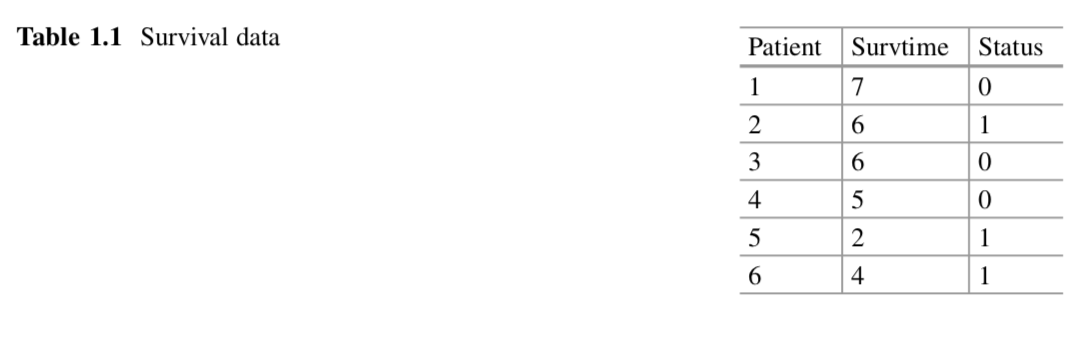
\includegraphics[scale = .35]{001.png}
\end{figure}
\end{frame}

\section{Case Deletion Residuals}
\begin{frame}[fragile]
\frametitle{Case Deletion Residuals}
\begin{itemize}
\item Some subjects may have an \empr{especially large influence} on the parameter estimates and may cause problems, so we have to identify them.
\item \empr{Case deletion residuals} (also called ``jackknife residuals'') serve this purpose.
\begin{defblock}{Case Deletion Residuals}
For each subject, a case deletion residual is the \empr{difference} in the value of the coefficient using all of the data and its value when that \empr{subject is deleted} from the data set.
\end{defblock}
\begin{Verbatim}
> result.coxph <- coxph(Surv(ttr, relapse) ~ grp + employment 
+ age)
> coef.all <- result.coxph$coef[4]
> coef.all
        age
-0.03528934
\end{Verbatim}
\end{itemize}
\end{frame}

\pagebreak
\begin{frame}[fragile]
\frametitle{Delete}
\begin{itemize}
\item For each subject in turn (``\texttt{n.obs}'' subjects in all), we delete the $i$th subject from the survival time ``\texttt{tt}'', censoring indicator ``\texttt{relapse}'', and covariates ``\texttt{grp}'', ``\texttt{employment}'', and ``\texttt{age}''
\item Fit a Cox model to this reduced data set. The results for the $i$th subject go into ``\texttt{result.coxph.i}''
\item Extract the age coefficient(4th) into ``\texttt{coef.i}'' and compute the jackknife residual as the difference of ``\texttt{coef.i}'' and ``\texttt{coef.all}'':
\begin{Verbatim}
> n.obs <- length(ttr)
> jkbeta.vec <- rep(NA, n.obs)
> for (i in 1:n.obs) \{
tt.i <- ttr[-i]
delta.i <- relapse[-i]
grp.i <- grp[-i]
employment.i <- employment[-i]
age.i <- age[-i]
result.coxph.i <- coxph(Surv(tt.i, delta.i) ~ grp.i +
employment.i + age.i)
coef.i <- result.coxph.i$coef[4]
jkbeta.vec[i] <- (coef.all - coef.i)\}
\end{Verbatim}
\end{itemize}
\end{frame}

\pagebreak
\begin{frame}[fragile]
\frametitle{Plot}
\begin{itemize}
\item Plot these residuals versus the patient id's, which we place in the vector ``\texttt{index.obs}'', ``\texttt{type='h'}'' causes the residuals to be plotted as spikes. ``\texttt{abline(h=0)}'' plots a horizontal line through 0.
\begin{Verbatim}
> index.obs <- 1:n.obs
> plot(jkbeta.vec ~ index.obs, type="h",xlab="Observation", 
ylab="Change in coefficient for age", cex.axis=1.3, cex.lab=1.3)
> abline(h=0)
\end{Verbatim}
\item The ``\texttt{identify}'' function allows us to identify the index numbers of select patients by manually selecting them with a mouse
\begin{Verbatim}
> identify(jkbeta.vec ~ index.obs)
\end{Verbatim}
\end{itemize}
\end{frame}

\pagebreak
\begin{frame}
\frametitle{Conclusion}
\begin{figure}
	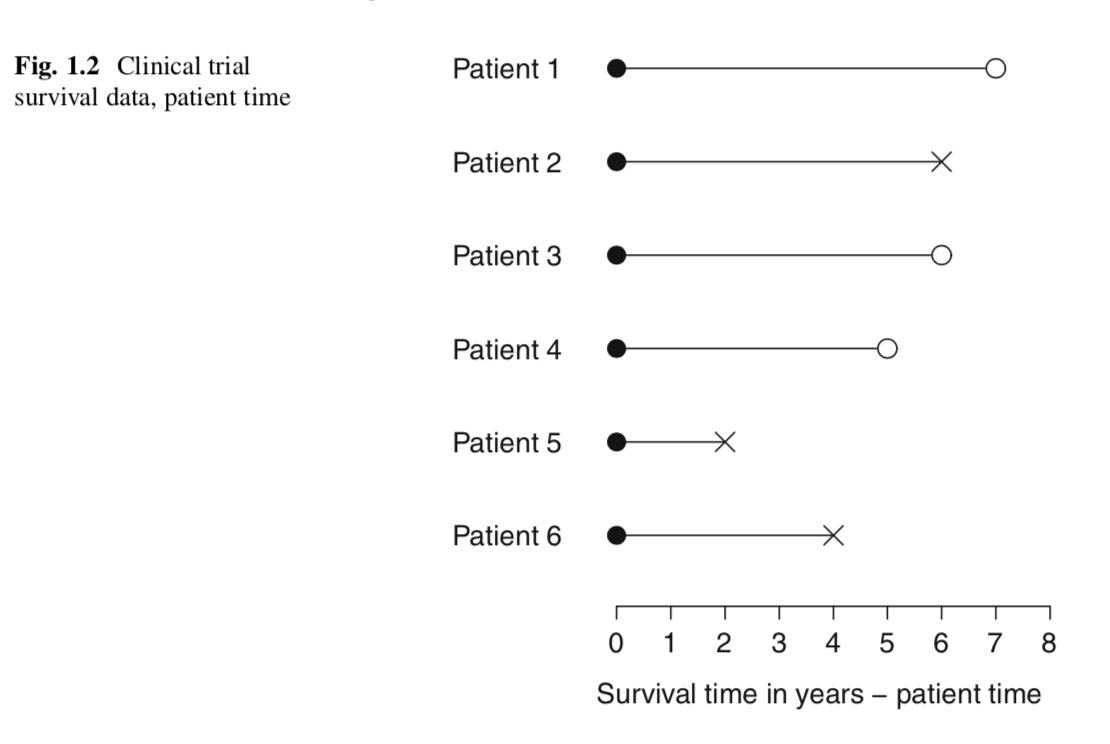
\includegraphics[scale = .4]{002.png}
\end{figure}
\begin{itemize}
\item Conclusion: No single patient changes the estimate of the ``\texttt{age}'' coefficient by more than 0.003, which is less than $10\%$ of the value of that coefficient. and patients 46 and 68 have the most influence over the parameter estimate for age.
\item A more convenient way to obtain case deletion residuals is using the ``\texttt{residuals}'' function with ``\texttt{type = 'dfbeta'}''.
\end{itemize}
\end{frame}

\pagebreak
\begin{frame}[fragile]
\frametitle{\texttt{debeta} residuals}
\begin{itemize}
\begin{Verbatim}
> resid.dfbeta <- residuals(result.coxph, type="dfbeta") 
> n.obs <- length(ttr)
> index.obs <- 1:n.obs
> plot(resid.dfbeta[,4] ~ index.obs, type="h",xlab="Observation", 
ylab="Change in coefficient") 
> abline(h=0)
> identify(resid.dfbeta[,4] ~ index.obs)
\end{Verbatim}
\item The resulting \texttt{dfbeta} residuals plot (not shown) is nearly \empr{identical}, it has the advantage that it is slightly easier to use it to produce multiple plots for all of the coefficients. 
\end{itemize}
\end{frame}


\section{Checking the Proportion Hazards Assumption}
\begin{frame}
\frametitle{Log Cumulative Hazard Plots}
\begin{itemize}
\item log-log transformation:
\begin{itemize}
\item Under the assumption, we have 
	\begin{equation}
	S_1(t) = [S_0(t)]^{exp(\beta)}
	\end{equation}
where $exp(\beta)$ is the proportional hazards constant.
\item Take logs both sides
\begin{equation}
\log[S_1(t)] = exp(\beta)\cdot \log[S_0(t)]
\end{equation}
\item The survival functions are less than 1, so log will cause negative.
\end{itemize}
\begin{equation}
\log \lbrace -\log[S_1(t)]\rbrace = \beta + \log \lbrace -\log[S_0(t)]\rbrace
\end{equation}
where the function $g(\mu) = \log \lbrace -\log(\mu) \rbrace$ is called a \empr{complementary log-log transformation}.
\item Plot $g[S_1(t)]$ and $g[S_0(t)]$ versus $t$ or $\log(t)$ will yield \empr{two parallel curves} separated by $\beta$ if the proportional hazards assumption is correct.
\end{itemize}
\end{frame}

\pagebreak
\begin{frame}[fragile]
\frametitle{Example}
\begin{itemize}
\item Illustrate this with the pancreatic cancer data from Chapter 3.
\begin{Verbatim}
# Plot the LA(Locally advanced)
> result.surv.LA <- survfit(Surv(pfs.month) ~ stage,
subset={stage == "LA"})
> time.LA <- result.surv.LA$time
> surv.LA <- result.surv.LA$surv
> cloglog.LA <- log(-log(surv.LA))
> logtime.LA <- log(time.LA)

# Plot the M(Metastatic)
> result.surv.M <- survfit(Surv(pfs.month) ~ stage, 
subset={stage == "M"})
> time.M <- result.surv.M$time
> surv.M <- result.surv.M$surv
> cloglog.M <- log(-log(surv.M))
> logtime.M <- log(time.M)
> plot(cloglog.LA ~ logtime.LA, type="s", col="blue", lwd=2)
> lines(cloglog.M ~ logtime.M, col="red", lwd=2, type="s")
> legend("bottomright", legend=c("Locally advanced",
"Metastatic"), col=c("blue","red"), lwd=2)
\end{Verbatim}
\end{itemize}
\end{frame}

\pagebreak
\begin{frame}
\frametitle{Example}
\begin{figure}
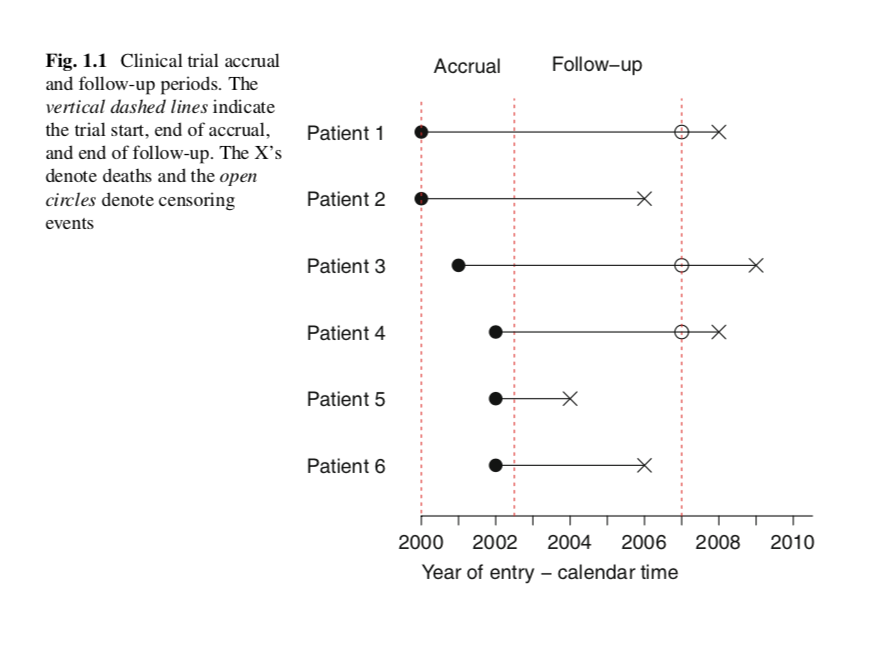
\includegraphics[scale = .35]{003.png}
\end{figure}
\begin{itemize}
\item Conclusion: The curves are clearly \empr{not parallel}. However, one problem with this approach is that we don't have a clear way to assess \empr{statistical significance}. This is a critical issue here due to the \empr{small sample size}, particularly in the locally advanced group.
\end{itemize}
\end{frame}

\section{Schoenfeld Residuals}
\begin{frame}
\frametitle{Recall}
\begin{itemize}
\item \empr{The Schoenfeld residuals} are the individual terms of \empr{the score function}, and each term is the observed value of the covariate for patient $i$ minus the expected value $E(Z_i) = \bar{z}(t_i)$, which is \empr{a weighted sum}, with weights given by $p_k(\beta)$, of the covariate values for subjects at risk at that time.
\item Recall:
\begin{itemize}
	\item The partial log-likelihood function
	\begin{equation}
	\ell(\beta) = \sum\limits_{i\in D }^{}\bigg\lbrace \log(\psi_i) - \log \bigg( \sum\limits_{k\in R_i }^{} \psi_k \bigg) \bigg\rbrace = \sum\limits_{i\in D }^{}\bigg\lbrace z_i\beta - \log \bigg( \sum\limits_{k\in R_i }^{} e^{z_k\beta} \bigg) \bigg\rbrace
	\end{equation}
	\item The score function:
		\begin{equation}
	\ell^{'}(\beta) = \sum\limits_{i\in D }^{}\bigg\lbrace z_i - \sum\limits_{k\in R_i }^{}z_k\cdot p(\beta,z_k) \bigg\rbrace  where \ p(\beta, z_k) = \frac{e^{z_k\beta	}}{\sum\limits_{j\in R_k}{}e^{z_j\beta}}  
	\end{equation}
\end{itemize}
\end{itemize}
\end{frame}


\pagebreak
\begin{frame}[fragile]
\frametitle{Example}
\begin{itemize}
\item For an estimate $\hat{\beta}$ the residual for the $i$th failure time is:
\begin{equation}
\hat{r_i} = z_i - \sum\limits_{k\in R_i}^{}z_k\cdot p(\hat{\beta},z_k) = z_i-\bar{z}(t_i)
\end{equation}
\item Example:
\begin{Verbatim}
> tt <- c(6, 7, 10, 15, 19, 25)
> delta <- c(1, 0, 1, 1, 0, 1)
> trt <- c(0, 0, 1, 0, 1, 1)
> result.coxph <- coxph(Surv(tt, delta) ~ trt) 
> result.coxph$coef
[1] trt -1.326
\end{Verbatim}
\item We see that $\hat{\beta}=1.326$. To compute the Schoenfeld residuals, we first compute the weights as follows:
\end{itemize}
\begin{figure}
	\includegraphics[scale = .35]{004.png}
\end{figure}
\end{frame}

\pagebreak
\begin{frame}[fragile]
\frametitle{Example}
\begin{itemize}
\item Compute the expected values, and then the residuals:
\begin{figure}
	\includegraphics[scale = .4]{005.png}
\end{figure}
\item In \texttt{R}:\linebreak
\begin{Verbatim}
> residuals(result.coxph, type="schoenfeld") 
[1]   6       10          15        25
-0.2098004 0.5566351 -0.3468347 0.0000000
\end{Verbatim}
\end{itemize}
\end{frame}

\pagebreak
\begin{frame}[fragile]
\frametitle{The scaled residual}
\begin{itemize}
\item Gramsch and Therneau proposed scaling each residual by an estimate of its variance. This \empr{scaled residual} conveniently approximated as follows:
\begin{equation}
r_{i}^{\star} = r_i\cdot d\cdot var(\hat{\beta})
\end{equation}
where $d$ is the total number of deaths, and $var(\hat{\beta})$ is the variance of the parameter estimate.
\end{itemize}
\begin{Verbatim}
> resid.unscaled <- residuals(result.coxph, type= ``schoenfeld'') 
> resid.scaled <- resid.unscaled*result.coxph$var*sum(delta)
> resid.unscaled
[1]      6        10        15         25 
   -0.2098004 0.5566351 -0.3468347 0.0000000
> resid.scaled
[1] -1.313064 3.483776 -2.170712 0.000000
\end{Verbatim}
\end{frame}


\pagebreak
\begin{frame}[fragile]
\frametitle{The scaled residuals}
\begin{itemize}
\item An approximate estimate of $\beta(t)$ may be obtained by adding the estimate $\hat{\beta}$ from the Cox proportional hazards model to the standardized residuals.
\begin{Verbatim}
> resid.scaled + result.coxph$coef
[1] -2.639193 2.157647 -3.496841 -1.326129
# or using ``cox.zph'' function
> resid.sch <- cox.zph(result.coxph)
> resid.sch$y
       trt
6  -2.639193
10  2.157647
15 -3.496841
25 -1.326129
\end{Verbatim}
\end{itemize}
\end{frame}

\pagebreak
\begin{frame}[fragile]
\frametitle{Example}
\begin{itemize}
\item Using this residuals to the pancreatic data, compute the \empr{scaled Schoenfeld residuals} and plot
\begin{Verbatim}
> result.coxph <- coxph(Surv(pfs.month) ~ stage)
#The ``transform'' option specifies that the time axis is scaled 
to conform with Kaplan- Meier-transformed time.
> result.sch.resid <- cox.zph(result.coxph, transform="km")]
> plot(result.sch.resid)
\end{Verbatim}
\end{itemize}
\begin{figure}
	\includegraphics[scale = .38]{006.png}
\end{figure}
\end{frame}

\pagebreak
\begin{frame}[fragile]
\frametitle{Example}
\begin{itemize}
\item The shape of the \empr{smoothed(loess) curve} is an estimate of the difference parameter as a function of time.
\item The hypothesis test for a constant $\beta$
\begin{Verbatim}
> result.sch.resid
         rho   chisq     p
stageM -0.328  3.86   0.0496
\end{Verbatim}
\item Alternatively, variations of this test may be obtained by plotting $\beta(t)$versus time or versus other transformations of time, and the ``\texttt{cox.zph}'' function offers:
\begin{itemize}
\item ``\texttt{rank}'' option: the time axis is ordered by the ranks of the times.
\item ``\texttt{identity}'' option: the time variable is untransformed.
\end{itemize}
\begin{Verbatim}
> cox.zph(result.coxph, transform="rank")
         rho    chisq     p
stageM  -0.33    3.89   0.0486
> cox.zph(result.coxph, transform="identity")
         rho    chisq     p
stageM  -0.197   1.39   0.239
\end{Verbatim}
\end{itemize}
\end{frame}
\end{document}